%\part*{Combinatorial Graph Algorithms}

%\epigraph{``It's game over now.''}{-- viš. znan. sod. dr. Rafael
%Benedikt Andrist}

\section{Classical Algos for Max Flow 1}

\datum{2026-05-05}


\begin{definicija}
    Consider a directed graph $G = (V,E,\mathbf{c})$, where $V$ are vertices, $E$ are edges and $\mathbf{c} \in \R_{\geq0} ^E$ denote edge capacities (imagine highway lanes with capacities in each direction and those capacities might be different).

    A \emph{flow} is any vector $f\in \R ^E$, but it is \emph{feasible} only if $\mathbf{0 \leq f \leq c}$, so if the flow respects directions and capacities.

    Again we define the edge-vertex incidence matrix $\mathbf{B} \in \R ^{V \times E}$ as 
    \begin{align*}
        \mathbf{B}(v, e) = \begin{cases} 
            1 & e = (u,v) \\
            -1 & e = (v, u)\\
            0 & else
        \end{cases}
    \end{align*}

    And here the signs are actually determined by the orientation.

    \emph{A demand vector} is any vector $\mathbf{d} \in \R ^V$ and $\mathbf{f}$ routes demand $\mathbf{d}$ if $\mathbf{Bf} = \mathbf{d}$

    here we focus on \emph{s-t flows}, which have the demand vecotr of the form $F(-\mathbf{e}_s + \mathbf{e}_t) =F \mathbf{b}_{st}$ for some scalar $F$. \textit{S} denotes the source, and \textit{T} denotes the sink (remember that S and T are consecutive letters, so it goes from S to T, negative means that it is a source, because it leaves the vertex and positive is a sink because it accumulates at the vertex). The vector $\mathbf{b}_{st}$ is just the vector with $-1$ at source and $1$ at sink.
\end{definicija}


Maximum flow can now be expressed as

\begin{align}
    \max_{\mathbf{f} \in \R ^E}  \quad &F \\
    \text{with } &\mathbf{Bf =} F \mathbf{b_{st}}, \, 0\leq \mathbf{f \leq c}
\end{align}

And we denote $val(\mathbf{f})$ the value of $F$ when $\mathbf{Bf} = F \mathbf{b}_{st}$.

So if $\mathbf{f}$ actually routes the \textit{s-t} flow, the scalar $F$ tells us how much of it we are currently routing. Without the upper constraint with $\mathbf{c}$ we could route infinite, but the upper constraint is what makes the problem interesting.

One obvious observation is that the max flow is achieved when at least one of the capacities is full.

\subsection{Flow decomposition}
We will try to simplify some flows
\begin{definicija}
    An \emph{s-t path flow} is a flow $\mathbf{f}\geq 0$ that can be written as 
    \begin{align*}
        f = \alpha \sum_{e \in p} \mathbf{e}_e
    \end{align*}
    where $p$ is a path from $s$ to $t$. So we only take a path and route all the demand on the path.
\end{definicija}

\begin{definicija}
    A \textit{cycle flow} is a path flow where $s = t$.
\end{definicija}

\begin{lema}[Path-cycle decomposition]

Any $s-t$ flow can be decomposed into a sum of $s-t$ path flows and cycle flows such that the sum contains at most $\text{nnz}(\mathbf{f})$ terms, where $\text{nnz}$ denotes the number of nonzero elements.

There is an optimal flow that contains only paths and no cycles in the decomposition.
    
\end{lema}

\begin{proof}
    We just take an $s-t$ path, get the minimal element and take the path with every element being the minimal and then we still end up with and $s-t$ flow but we now have another zero element in the rest. We can also do this thing with the cycle.

    And it is obvious that we must either have a path or a cycle always, because routing only goes from $s$ to $t$ and can't accumulate anywhere else.

    In the optimal case if we have a cycle it is not helping route any demand so we delete it and still get flow which routes the same demand, but the flow is strictly smaller.
\end{proof}

We do know that the optimal flow might not be unique, even without the cycles, just imagine $A \rightarrow B \rightarrow C \rightarrow D$ with an additional edge from $A$ to $C$.


\subsection{Cuts and Minimum Cuts}

From the previous decomposition we can see that if we take a cut that separates $S$ and $T$ we see that the max flow can route at most the demand of the edges contained in the cut. And if we take the minimum we get that the max flow is atmost the minimum of the cut.



\begin{definicija}
    Given a vertex subset $S \subset V$ we say that $(S, V \setminus S)$ is a \emph{cut} in $G$ and that the value of the cut is 
    
    \begin{align}
        c_G (S) = \sum_{e\in E \cap (S \times V \setminus S) } \mathbf{c(e)}
    \end{align}

    In the directed graphs, only the edges crossing in the right direction count (from set $S$ away.
\end{definicija}

\begin{definicija}
    And \emph{s-t cut} is a cut where $s \in S$ and $t \in V\setminus S$
\end{definicija}

\begin{izrek}
    For any \textit{s-t flow} $\mathbf{f}$ and \textit{s-t cut} $S$ we have
    \begin{align}
        \text{val}(\mathbf{f}) \leq c_G(S)\\
        \textbf{max flow} \leq \textbf{min cut}
    \end{align}
\end{izrek}

\obvs


\subsection{Algos for Max flow}

\begin{algorithm}
\caption{First try at algo}\label{alg:first}
\begin{algorithmic}
\State $\mathbf{f} \gets 0$
\While{}\\
    Find \emph{s-t} path flow that is feasible wrt to $\mathbf{c - f}$
    \State $ \mathbf{f} \gets \mathbf{f + \Tilde{\mathbf{f}}}$
\EndWhile
\end{algorithmic}
\end{algorithm}

This is a primitive algorithm that doesn't always find the optimal path. 

Consider a graph on 4 vertices $A, B ,C ,D$ with edges $(A,B), (A,C), (B, C), (B,D), (C,D)$ with all edges having the same capacity $1$. If we take the path $ABCD$ we are left only with edges $AC$ and $BD$ and we can't find a path, but we didn't find the max flow.

\begin{figure}[h]
\centering
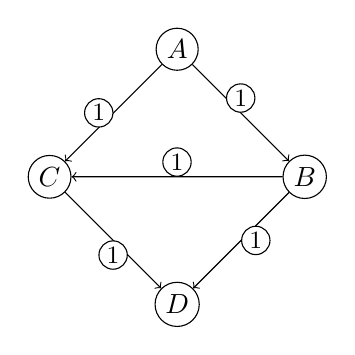
\begin{tikzpicture}[
  scale=1.35,
  every node/.style={circle,draw,inner sep=1.8pt},
  edge label/.style={midway,fill=white,inner sep=1pt,font=\small}
]
  \node (A) at (0,2.4) {$A$};
  \node (B) at (1.2,1.2) {$B$};
  \node (C) at (-1.2,1.2) {$C$};
  \node (D) at (0,0) {$D$};

  % all capacities are 1
  \draw[->] (A) -- node[edge label,above] {$1$} (B);
  \draw[->] (A) -- node[edge label,left]  {$1$} (C);
  \draw[->] (B) -- node[edge label,right] {$1$} (D);
  \draw[->] (C) -- node[edge label,below] {$1$} (D);
  \draw[->] (B) -- node[edge label,sloped,above] {$1$} (C);
\end{tikzpicture}
\caption{Example where greedy augmentation along $A\to B\to C\to D$ gets stuck.}
\end{figure}

We can try to fix this by basically adding reverse edges for the path $\mathbf{f}$. So here we would then add edges $DC, CB, BA$ all with capacity $1$ and repeat the algorithm and then we can find a path $ACBD$ and when summing those up we see that the edge $BC$ gets used in both direction, so it is basically at $0$.

More formally we do it like this

\begin{algorithm}
\caption{Second try at algo}\label{alg:second}
\begin{algorithmic}
\State $\mathbf{f} \gets 0$
\While{}\\
    Find \emph{s-t} path flow $\Tilde{\mathbf{f}}$ that is feasible wrt to $ - \mathbf{f} \leq \Tilde{\mathbf{f}} \leq \mathbf{c - f}$
    \State $ \mathbf{f} \gets \mathbf{f + \Tilde{\mathbf{f}}}$
\EndWhile
\end{algorithmic}
\end{algorithm}

And we say we are doing this with residual graphs. We actually don't get the exact same thing that I said, here we don't respect the thing that we actually might have the edges going back in that direction anyway, but it should be essentially the same kinda.

The residual graph is denoted by $G_f$ and it is only defined for feasible $\mathbf{f}$. An edge with $\ff (e) = \ccc$ is called \emph{saturated}. 

\begin{lema}
    Suppose $\Tilde{\ff}, \ff$ arre feasible in $G$, then $\Tilde{\ff} - \ff$ (where negatives count as flow in opposite direction) is feasible in $G_f$.
\end{lema}

\obvs

\begin{lema}
    Suppose $\ff$ is feasible in $G$ and $\Tilde{\ff}$ is feasible in $G_f$, then $\ff + \Tilde{\ff}$ is feasible in $G$.
\end{lema}

\obvs

\begin{lema}
    A feasible $\ff$ is optimal $\iff$ $t$ isn't reachable from $s$ in $G_f$.
\end{lema}

\obvs

From this we can actually get that the max flow is equal to the min cut.

\begin{izrek}[Max Flow = Min Cut]
    The maximal flow equals the minimum cut.
\end{izrek}

\begin{proof}
    Consider $G_f$ for a maximal flow. Then there is no path from $s$ to $t$ and thus we have used all the edges from some cut.
\end{proof}


Note that this proof gives an algorithm to calculate the min cut from the $s-t$ maximum flow (take vertices reachable from $s$ in the residual graph).


\begin{algorithm}
\caption{Ford-Fulkerson Algo}\label{alg:second}
\begin{algorithmic}
\State $\mathbf{f} \gets 0$
\While{}\\
    Find any $s-t$ path flow in $G_f$ and add it to $\ff$.
\EndWhile
\end{algorithmic}
\end{algorithm}

Does it always converge? For integers/rationals yeah in finite time, but for irrationals it might not terminate, and even might not converge at all (There is an example on wikipedia, I didn't really check it out tho).

\begin{lema}
    Consider Ford-Fulkerson algo with integer capacities. The algorithm terminates i $\text{val}(\ff)$ augmentations, so $O(|E| \text{val} \ff)$ time.
\end{lema}

\begin{proof}
    Each iteration will increase it by an integer and we will always be able to increase it until we get max flow. And each iteration can be computed in $O(|E|)$ time. We start from $s$ and go to the neighbours and only keep the account of the max flow we can get to a vertex (or the first) (breadth or depth first search uses $O(m+n) = O(m)$ as $m>n-1$ from connected graph).
\end{proof}


We can try to improve the algorithm by trying to binary search the maximum bottleneck capacity instead of just using any capacity we find. So for a fixed capacity we take only the edges that carry atleast that capacity and observe if we can get accross. This can be done in $O(m)$ and binary search in $O(n)$, but we also know that since we saturated atleast one edge, the path must carry atleast $\frac 1 m$ of the flow left in $G_f$, so we now have anther bound on how fast this will converge. The algorithm thus for sure converges when

\begin{align*}
    (1 - \frac 1 m) ^T \text{val}(\ff) <1
\end{align*}

where $T$ denotes the number of iterations.

We can approximate $\ln (1-\frac 1 m) \approx -1/m$ and get that $T \approx m \ln F$ suffices.

So we get the total time to be

\begin{align}
    O(m T \ln n) = O(m ^2 \ln F \ln n) \leq O(m^2 \ln n \ln (m \max (c)))
\end{align}

For integer capacities the state of the art achieves $O(m^{1 + o(1)}) \ln (U)$ where $U$ is the max capacity. For real valued capacities it is $O(mn)$ by Orlin (thats whats in the script).











